\section{System Design}
In this section we elaborate the underling system design which is capable of processing 2.4 million messages per second. We emphazise three features of this design. Firstly between any two nodes there is a set of tcp connections (typically 20 connections)  to send messages. All processes share the same set of connections which we called as the bridge. The advantage of this approach compared to having tcp connections per process is that it utilizes all available bandwidth even there is only one process per node. However since this is a common bridge now we need to send receiving process id to dispatch the message, sending  process id to parse the message and sequence number to order messages. As we show latter our experiments shows this approach perform several times better than the other systems dispite above overhead. Secondly we have implemented java.io.OutputStream and java.io.InputStream interfaces on top of java.nio API. Using these input and output streams we provide java.io.DataOutput and java.io.
DataInput 
objects to directly serialize message data to binary format to without sending any metadata along the message. As we explained in earlier section our Event interface provides these methods. Finally except messages itself all the other objects used to send the messages and parse the messages are not created at message processing time. When a process sends the first message all these objects are created and it is a one time cost. Rest of this section further explain how we have implemented above techniques.
\subsection{Inter Process Communication}
Figure \ref{interprocess} shows the design involves in sending a message from one process to another. Lets assume there is a message object at a client side process and that process wants to send this message to another process. First client process sends this message to its ElementContainer. ElementContainer holds all the streams (this is an abstraction of a link in the process graph) to which this message needs to send and it push the message to all streams. Stream object decides which node to send this message and pass the message along the taget node details to ConnectionManager which holds ClientConnection object for each node. ConnectionManager picks the correct ClientConnection for target node and sends the message to ClientConnection. ClientConnection picks an available DataOutput object and invokes the serialize method of the message to send that to server side.

At the server side there are a set of ServerTasks which read receiving messages at DataInput streams available in the ServerConnection (we register these connections at the connections creating time). Once a server task receives a binary message, it creates the event object using the sending process id to identify the event type. Then it pass this message to the WorkerContainer which holds all processes. Finally WorkerContainer dispatch this message to correct process uisng receiving process id. Message ordering happens at the process level if required. This elastrates how we have shared a pool of tcp connections among process and next we show how we have implemented java.io.OutputStream and java.io.InputStream without creating objects dynamically. 
\begin{figure}[!t]
        \centering
        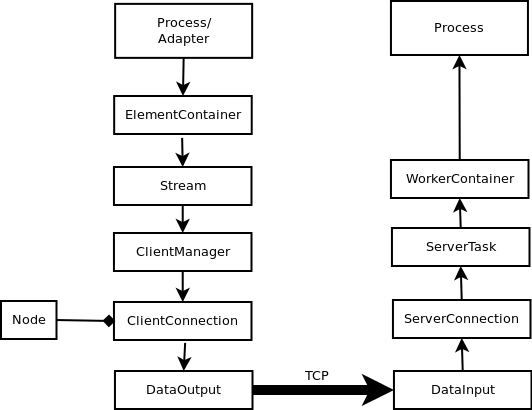
\includegraphics[width=3.0in]{interprocess.png}
        \caption{Communication between two Process}
        \label{interprocess}
\end{figure}
\subsection{Client Side}
Figure \ref{client} shows how we have implemented java.io.OutputStream interface using our DataWriter class. DataWriter contains a java.nio.ByteBuffer object. When a higher layer method writes data to DataOuput object, DataWriter put those bytes to its byte buffer. When a selection event occurs, Datawriter writes its byte buffer to under line SocketChannel. This way we use one byte buffer as a intermediatory create an output stream with java.nio API.
\begin{figure}[!t]
        \centering
        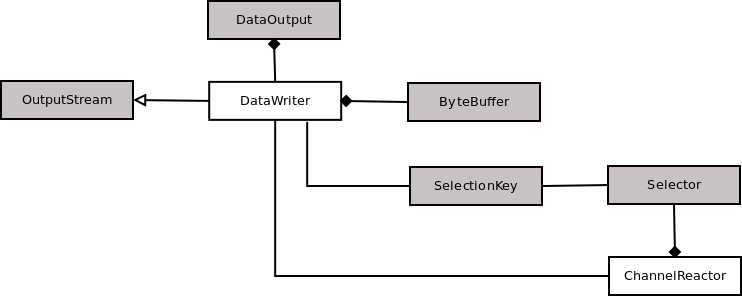
\includegraphics[width=3.0in]{client.png}
        \caption{OutputStream Implementation}
        \label{client}
\end{figure}
\subsection{Server Side}
Figure \ref{server} shows how we have implemented java.io.InputStream interface using our DataReader class. Similar to clinet side, DataReader object has a java.nio.ByteBuffer object. When a selection event occurs DataReader input bytes from the SocketChannel to its byte buffer. When a ServerTask reads data through DataInput, it reads data from the byte buffer and passes to higher layer. In this way we have implemented an input stream with java.nio API.
\begin{figure}[!t]
        \centering
        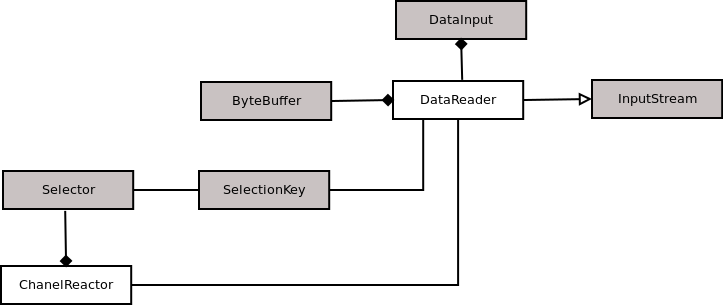
\includegraphics[width=3.0in]{server.png}
        \caption{InputStream Implementation}
        \label{server}
\end{figure}
